\documentclass[a4paper,10pt]{article}

\usepackage{ucs}
\usepackage[utf8x]{inputenc}
\usepackage{amsmath}
\usepackage{amsfonts}
\usepackage[french]{babel}
\usepackage{xcolor}
\usepackage{fontenc}
\usepackage{graphicx}
\usepackage{caption}
\usepackage{subcaption}
\usepackage{amsthm}
\usepackage{fancyhdr}
\usepackage{bm}
\usepackage{stmaryrd}

\pagestyle{fancy}

\renewcommand\headrulewidth{1pt}
\fancyhead[L]{ENSIMAG 1A 2019}
\fancyhead[R]{Méthodes Numériques}
\newtheorem{lemma}{Lemme}[section]
\newtheorem{remark}{Remarque}[section]
\newtheorem{definition}{Définition}[section]
\newtheorem{corollary}{Corollaire}[section]
\newtheorem{proposition}{Proposition}[section]
\newtheorem{theorem}{Théorème}[section]
\newtheorem{question}{Question}

\usepackage{hologo}
\usepackage[colorlinks = true,
            linkcolor = blue,
            urlcolor  = magenta,
            citecolor = blue,
            bookmarks=true,
            bookmarksnumbered=true,
            anchorcolor = blue]{hyperref}

\newcommand{\ttt}[1]{\texttt{#1}}
\newcommand{\correct}[1]{\textcolor{red}{{#1}}}
\newcommand{\scalar}[1]{#1}
\newcommand{\complex}[1]{\bm{#1}}
\renewcommand{\vec}[1]{\bm{#1}}
\newcommand{\R}{\mathbb{R}}
\newcommand{\N}{\mathbb{N}}
\newcommand{\C}{\mathbb{C}}
\newcommand{\I}{\complex{i}}
\newcommand{\kx}{\complex{k_x}}
\newcommand{\ky}{\complex{k_y}}
\newcommand{\kxq}{\complex{k_{x,q}}}
\newcommand{\kyp}{\complex{k_{y,p}}}
\renewcommand{\O}{\mathcal{O}}
\newcommand{\dft}[1]{\mathcal{F}{\left( #1 \right)}}
\newcommand{\dd}{\mathrm{d}}
\newcommand{\dt}{\dd\mathrm{t}}
\newcommand{\dx}{\dd\mathrm{x}}
\newcommand{\dy}{\dd\mathrm{y}}
\newcommand{\dnu}{\dd\mathrm{\nu}}
\newcommand{\dmu}{\dd\mathrm{\mu}}

% variables
\newcommand{\viscodynf}{\scalar{\eta}}
\newcommand{\viscocinf}{\scalar{\nu}}
\newcommand{\densf}{\scalar{\rho}}
\newcommand{\pos}{\vec{x}}
\newcommand{\vel}{\vec{u}}
\newcommand{\velh}{\hat{\vec{u}}}
\newcommand{\vort}{\vec{\omega}}     % 3D vorticity is a vector
\newcommand{\vorts}{\scalar{\omega}} % 2D vorticity is a scalar
\newcommand{\velx}{\vel_x}
\newcommand{\vely}{\vel_y}
\newcommand{\velz}{\vel_z}
\newcommand{\vortx}{\vort_x}
\newcommand{\vorty}{\vort_y}
\newcommand{\vortz}{\vort_z}
\newcommand{\velxh}{\velh_x}
\newcommand{\velyh}{\velh_y}
\newcommand{\x}{(\pos)}
\newcommand{\X}{x,y}
\newcommand{\xt}{(\pos,t)}
\newcommand{\Xt}{(\X,t)}

% opérateurs différentiels
\newcommand{\nablav}{\vec{\nabla}}
\newcommand{\ppd}[2]{\frac{\partial#1}{\partial#2}}
\newcommand{\pd}[2]{\dfrac{\partial#1}{\partial#2}}
\newcommand{\Dt}[1]{\pd{#1}{t}}
\newcommand{\Dx}[1]{\left(\vel\cdot\nablav\right) #1}
\newcommand{\D}[1]{\Dt{#1} + \Dx{#1}}
\newcommand{\grad}[1]{\nablav #1}
\renewcommand{\div}[1]{\nablav \cdot #1}
\newcommand{\curl}[1]{ \nablav \wedge #1 }
\newcommand{\laplacian}[1]{\Delta #1 }

% voir https://tex.stackexchange.com/questions/14071/how-can-i-increase-the-line-spacing-in-a-matrix
\makeatletter
\renewcommand*\env@matrix[1][\arraystretch]{%
  \edef\arraystretch{#1}%
  \hskip -\arraycolsep
  \let\@ifnextchar\new@ifnextchar
  \array{*\c@MaxMatrixCols c}}
\makeatother

% suppression des indentations automatiques
\setlength\parindent{0pt}

\begin{document}
  \begin{center}
     \begin{LARGE}
         \textbf{Rendu TP Méthodes Numériques~:}\\
         \textit{Simulation d'écoulement fluide}
     \end{LARGE}
 \end{center}
$$
$$
 \begin{center}
 \begin{LARGE}
    \text{Fait par: BCHIR Yousra, AIT LAHMOUCH
Nadir}
    \end{LARGE}
\end{center}
$$
$$
$$
\section{Résolution de l'équation de transport diffusion}
\begin{question}
Après des calculs pour résoudre le système:
\[
   N\left[\begin{array}{c}
          \phi(0,(k+1)\dt)\\
          \vdots\\
          \phi(n\dx,(k+1)\dt)\\
          \vdots\\
          \phi((N_x-1) \dx,(k+1)\dt)\\
  \end{array}\right]
 =M
  \left[\begin{array}{c}
          \phi(0,k\dt)\\
          \vdots\\
          \phi(n\dx,k\dt)\\
          \vdots\\
          \phi((N_x-1)\dx,k\dt)\\
  \end{array}\right]
\]
On arrive aux résultats suivants:
$$
N = \begin{pmatrix}
1 + 2\kappa \frac{\dt}{\dx^2}  &  -\kappa \frac{\dt}{\dx^2} & 0 &\dots&\dots &0  & -\kappa \frac{\dt}{\dx^2}
\\-\kappa \frac{\dt}{\dx^2} & \ddots & -\kappa \frac{\dt}{\dx^2} & 0 & \dots & \dots& 0 \\0&\ddots&\ddots&\ddots&\ddots&&\vdots\\\vdots&&&\croixdots&&&\vdots\\\vdots&\revdots&\revdots&&\ddots&\ddots&\vdots
\\0 & 0 & \revdots &&\ddots& 1 + 2\kappa \frac{\dt}{\dx^2} & -\kappa \frac{\dt}{\dx^2}
\\-\kappa \frac{\dt}{\dx^2}& 0 &\dots&\dots&\dots& -\kappa \frac{\dt}{\dx^2} & 1 + 2\kappa \frac{\dt}{\dx^2}
\end{pmatrix}
$$
$$
\hspace{-30mm}M = \left(\begin{smallmatrix}
1 -c(0)^2\frac{\dt^2}{\dx^2};  &  -c(\dx)\frac{\dt}{2\dx}+c(\dx)^2\frac{\dt^2}{2\dx^2} & 0 &\dots&0  & -c((N_x-1) \dx)\frac{\dt}{2\dx}+c((N_x-1) \dx)^2\frac{\dt^2}{2\dx^2}
\\ c(0)\frac{\dt}{2\dx}+c(0)^2\frac{\dt^2}{2\dx^2}& \ddots & \ddots & 0 & \dots& 0 \\0&\ddots&\ddots&\ddots&&\vdots
\\\vdots&\ddots&\ddots&&&\vdots
\\\vdots&\revdots&\revdots&&\ddots&0
\\0 & 0 & \revdots &&\ddots& -c((N_x-1)\dx)\frac{\dt}{2\dx}+c((N_x-1)\dx)^2\frac{\dt^2}{2\dx^2}
\\-c(0)\frac{\dt}{2\dx}+c(0)^2\frac{\dt^2}{2\dx^2}& 0 &\dots&\dots&c((N_x-2)\dx)\frac{\dt}{2\dx}+c((N_x-2)\dx)^2\frac{\dt^2}{2\dx^2}& 1 -c((N_x-1)\dx)^2\frac{\dt^2}{\dx^2}
\end{smallpmatrix}\right)
\end{question}
$$
$$
\hspace{-20mm}Les matrices $M$ et $N$ se sont pas tridiagonales par argument de périodicité.
$$
$$
$$
$$
\vskip 0.5cm

\begin{question}
on montre dans cette question que la matrice $N$ est symétrique (trivial) définie positive
\vskip 0.1cm
on pose: \alpha=\kappa \frac{\dt}{\dx^2} \: et \ un \ vecteur \ non \ nul \ $X$ \ :\  $X$=\left[\begin{array}{c}
          x_{0}\\
          x_{1}\\
          \vdots\\
          x_{N_x-1}\\
  \end{array}\right]
\vskip 0.2cm
et on montre que  ^tXNX  \: est \: strictement positif
\vskip
\begin{subequations}
\begin{eqnarray*}
\displaystyle
^tXNX=((1+2\alpha) x_{0}-\alpha x_{1}-\alpha x_{N_x-1})x_0+\sum_{1}^{N_x-2}((1+2\alpha)x_k-\alpha(x_{k-1}+x_{k+1}))x_{k}
\displaystyle

                &&+ (1+2\apha)x_{N_x-1}-\alpha(x_{N_x-2} + x_0)
\end{eqnarray*}
\end{subequations}
\vskip 0.2cm
alors
\begin{subequations}
\begin{eqnarray*}
\displaystyle
^tXNX=\sum_{k=0}^{N_x-1}x_k^2+2\alpha(\sum_{k=0}^{N_x-2}x_k^2-x_kx_{k+1})-2\alpha x_0x_{N_x-1} + 2\alpha x_{N_x-1}^2
\end{eqnarray*}
\end{subequations}
\vskip 0.2cm
donc
\begin{subequations}
\begin{eqnarray}
\displaystyle
^tXNX= \sum_{k=0}^{N_x-1} x_k^2 + \sum_{k=0}^{N_x-2}(x_k-x_{k+1})^2 + (x_0 -x_{N_x-1})^2
\end{eqnarray}
\end{subequations}
\vskip 0.2cm
Et comme \ $\sum_{k=0}^{N_x-1} x_k^2$ \ est forcément strictement positif, alors on déduit que N est bien symétrique définie positive.
\vskip 0.2cm
On a N symétrique définie positive, ceci justifie la possibilité d'utiliser la méthode de cholesky qui est deux fois plus rapide que la méthode de factorisation LU.
\end{question}
\vskip 1cm
\begin{question}
Dans cette question on nous demande de compléter le fichier "mycholesky.sce" pour implémenter une fonction qui renvoi la solution des équation de type NU = S, en utilisant la factorisation de cholesky, qui est connue pour son coût moindre et sa rapidité. La solution se trouve donc dans le dossier joint à ce rapport.
\end{question}
\vskip 8cm
\begin{question}
Après avoir implémenté la résolution de l'équation sur scilab de l'équation étudiée en utilisant la méthode demandée dans l'énoncé soit après sa discrétisation, on arrive aux résultats suivants.
\begin{center}
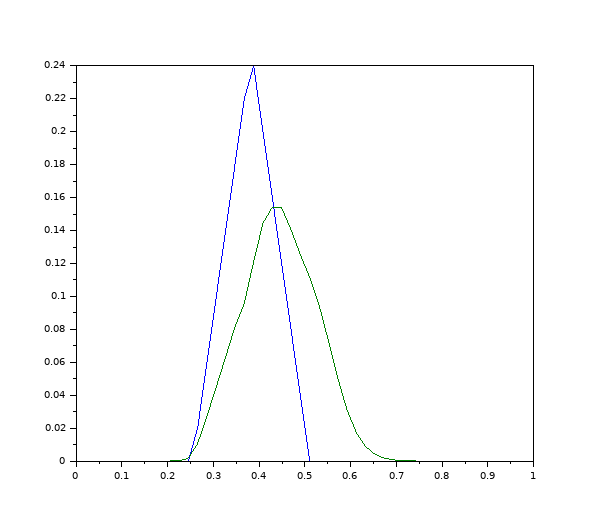
\includegraphics[scale=0.4]{k=00001.png}}
\captionof{figure}{Résultat avec kappa=0.0001}
\label{fig1}
\end{center}
\vskip 1cm
\begin{center}
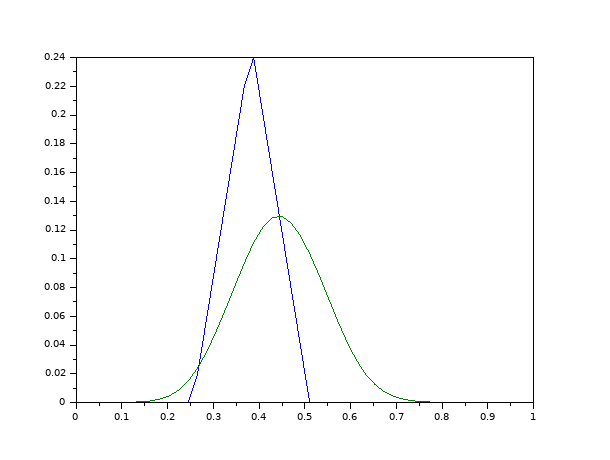
\includegraphics[scale=0.4]{k=0001.png}}
\captionof{figure}{Résultat avec kappa=0.001}
\label{fig2}
\end{center}
\vskip 2cm
\begin{center}
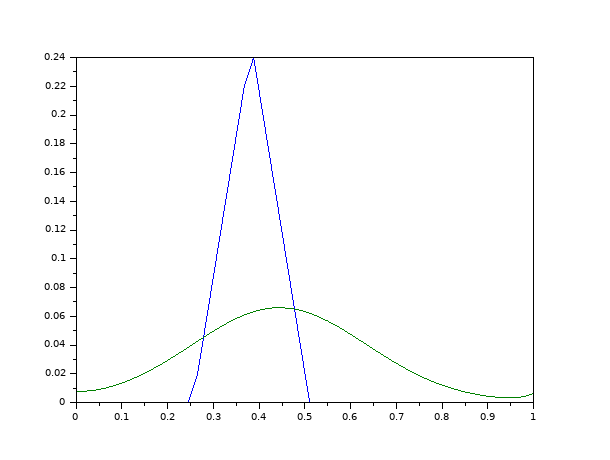
\includegraphics[scale=0.4]{k=001.png}}
\captionof{figure}{Résultat avec kappa=0.01}
\label{fig3}
\end{center}
\vskip 0.5cm
\textbf{On remarque que plus kappa est petit plus la solution Phi finale s'éloigne de son état initial, ce qui est normal.}
\end{question}
\vskip 1cm
\begin{question}
Dans cette question, on représentera à chaque pas de temps, les versions
discrétisées des fonctions scalaires par les tableaux $f^k_{i,j}\simeq f(j\dx,i\dy,k\dt)$.
On va appliquer les résultats trouvés en 1D en réalisant un splitting directionnel.
\vskip 0.2cm
\textbf{Après avoir remplacé le solveur 1D et implémenté le solveur 2D sur scilab, le test donne comme résultats:}
\begin{center}
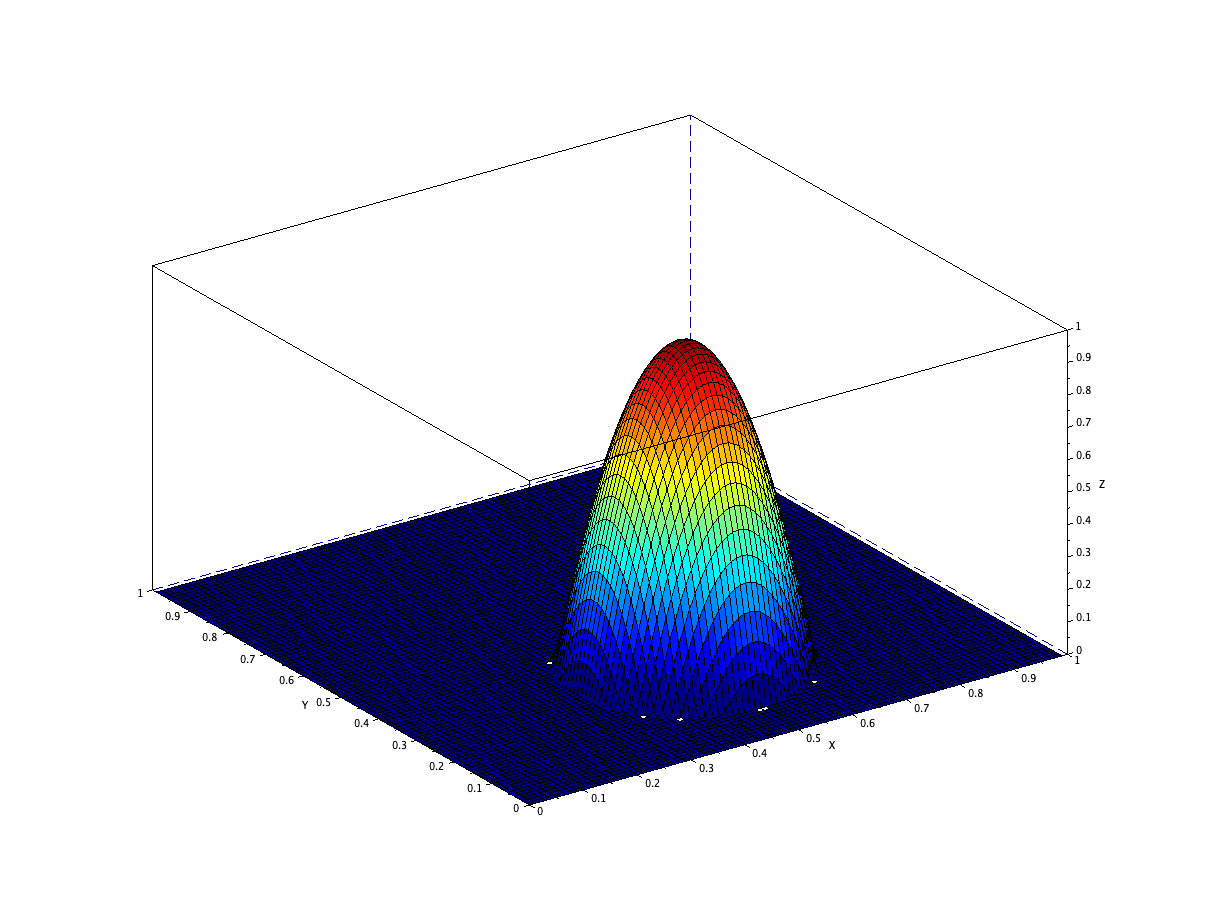
\includegraphics[scale=0.2]{qst5initial.png}}
\captionof{figure}{Résultat à l'instant initial}
\label{fig3}
\end{center}
\vskip 0.2cm
\begin{center}
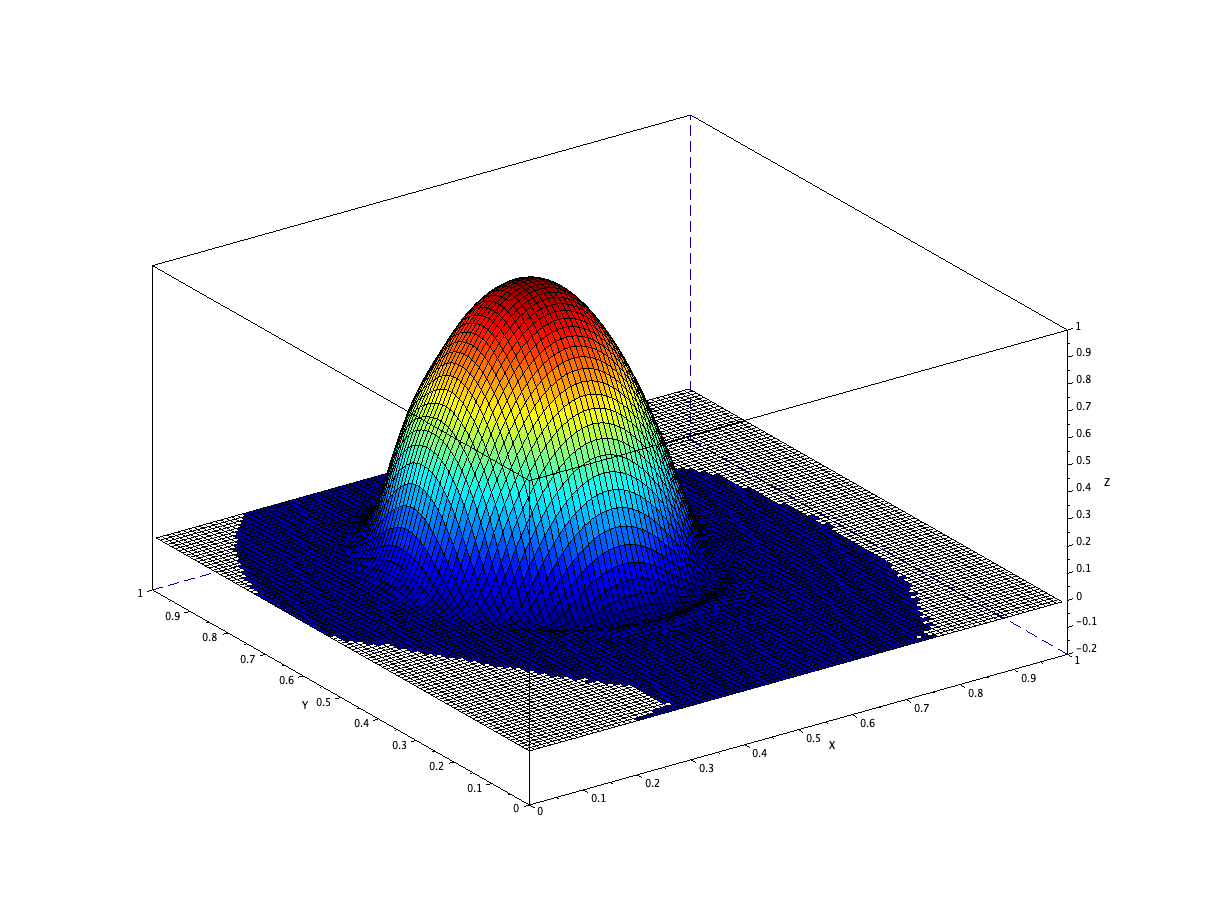
\includegraphics[scale=0.2]{qst5final.png}
\captionof{figure}{Résultat à l'instant final}
\label{fig3}
\end{center}
\vskip 0.2cm
Changeons maintenant la valeur de kappa pour voire si ce modèle suit la même conjecture établie dans le modèle à 1 seule dimension.
\begin{center}
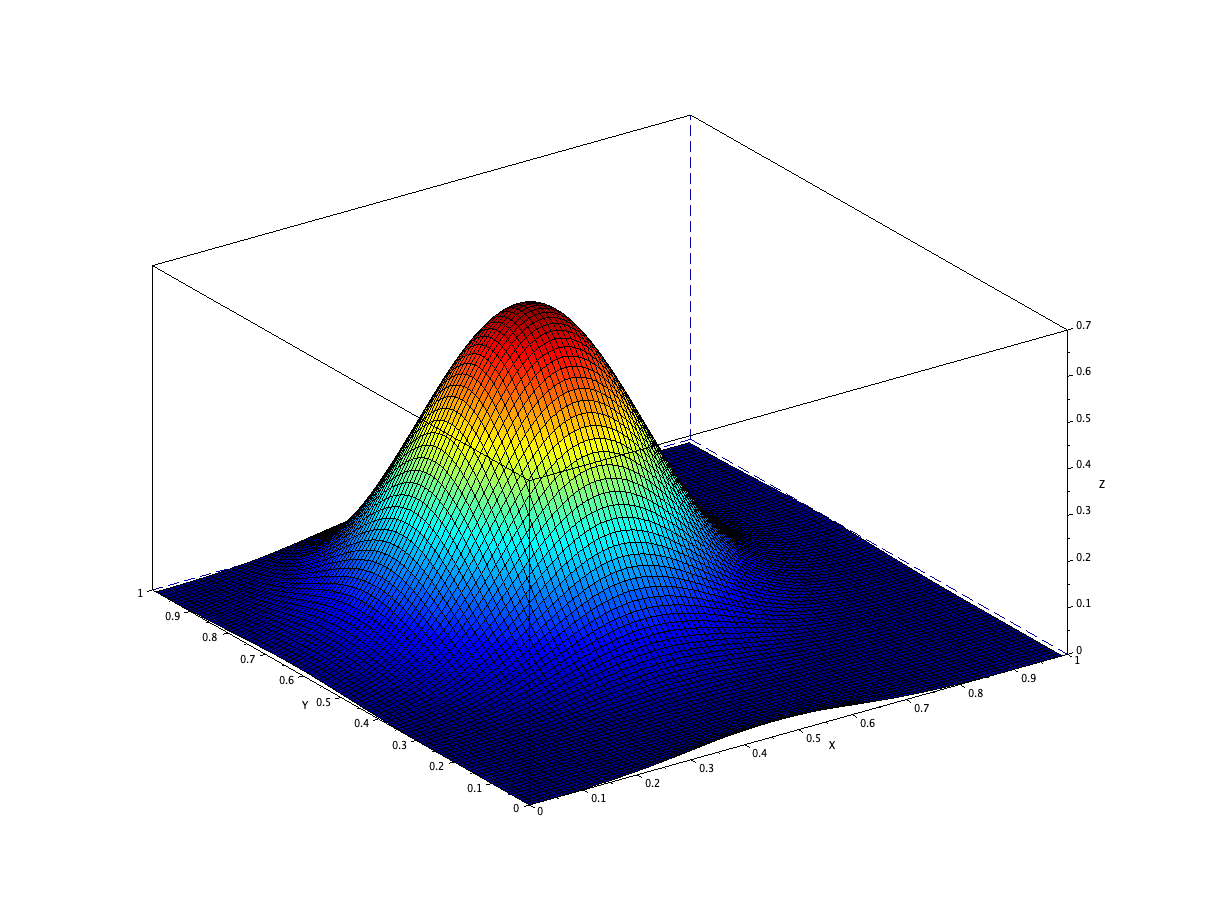
\includegraphics[scale=0.2]{qst5finale001.png}
\captionof{figure}{Résultat à l'instant final avec kappa=0.01}
\label{fig3}
\end{center}
\vskip 0.2cm
Effectivement, quand on augmente la valeur de kappa, la courbe tend à s'applatir sur les bords tout en diminuant en amplitude.
\vskip 0.2cm
\textbf{On remarque bien que le modèle 2D donne le même résultat que celui qu'avec une seule dimension.
Effectivement, la courbe à l'instant initial présente une courbe haute pointue qui s'applatit sur les bords tout en dimnuant en amplitude à l'instant final. Et cela en dépendant de la valeur de kappa choisie.
On pourrait en tirer exactement les mêmes résulats en intersectant un plan Z avec les courbes obtenues.}

\end{question}
\vskip 6cm
\section{Résolution du problème du poisson}
\vskip 0.5cm
\begin{question}
on a $ \frac{\partial\psi}{\partial x^2}(x,y)+ \frac{\partial \psi}{\partial y^2}(x,y) = f(x,y)$
\vskip 0.2cm
alors :
\begin{subequations}
$$S_{n m}( \frac{\partial\psi}{\partial x^2}) +S_{n m}( \frac{\partial \psi}{\partial y^2}) = S_{n m}(f)$$
\end{subequations}
\vskip 0.2cm
$$\frac{\partial S_{n m} (\psi)}{\partial x^2}+ \frac{\partial S_{n m}(\psi)}{\partial y^2} = S_{n m}(f)
$$

\vskip 0.2cm
on calcule $\frac{\partial S_{n m} (\psi)}{\partial x^2}$:

$$
\begin{aligned}
\frac{\partial S_{n m} (\psi)}{\partial x^2}
&= \frac{ \partial \sum\limits_{p = -n}^{p = n} \sum\limits_{q = -m}^{q = m} \hat{\psi}_{p q} \exp(+ k_y y) \exp( + k_x x)}{\partial x^2}  \\
&= \frac{ \partial \sum\limits_{p = -n}^{p = n} \sum\limits_{q = -m}^{q = m} k_x \hat{\psi}_{p q} \exp(+ k_y y) \exp( + k_x x)}{\partial x} \\
&= \sum\limits_{p = -n}^{p = n} \sum\limits_{q = -m}^{q = m} k_{x}^{2} \hat{\psi}_{p q} \exp(+ k_y y) \exp( + k_x x)
\end{aligned}
$$
\vskip 0.2cm
de même  pour $\frac{\partial S_{n m} (\psi)}{\partial x^2}$:

$$
\begin{aligned}
\frac{\partial S_{n m} (\psi)}{\partial y^2}
&= \frac{ \partial \sum\limits_{p = -n}^{p = n} \sum\limits_{q = -m}^{q = m} \hat{\psi}_{p q} \exp(+ k_y y) \exp( + k_x x)}{\partial y^2} \\
&= \frac{ \partial \sum\limits_{p = -n}^{p = n} \sum\limits_{q = -m}^{q = m} k_y \hat{\psi}_{p q} \exp(+ k_y y) \exp( + k_x x)}{\partial y} \\
&= \sum\limits_{p = -n}^{p = n} \sum\limits_{q = -m}^{q = m} k_{y}^{2} \hat{\psi}_{p q} \exp(+ k_y y) \exp( + k_x x)
\end{aligned}
$$
alors on trouve la relation suivante:
    $$ (k_{y}^{2} + k_{x}^{2}) \hat{\psi})_{p q} = \hat{f}_{p q}$$
\end{question}
\vskip 1cm
\begin{question}
on a
\[
\left \{
\begin{array}{c @{=} c}
    \Delta u_{x}(x,y) & - \frac{\partial \omega (x,y)}{\partial y}  \\
     \Delta u_{y}(x,y) &  \frac{\partial \omega (x,y)}{\partial x}
\end{array}
\right.
\]
de la même manière que la question 6, on trouve:
\[
\left \{
\begin{array}{c @{=} c}
    ( k_{x}^{2} + k_{y}{2}) \hat{u}_{x}_{p q} & - k_{y} \hat{\omega}_{p q }  \\
    ( k_{x}^{2} + k_{y}{2}) \hat{u}_{y}_{p q } &  k_{x} \hat{\omega}_{p q}
\end{array}
\right.
\]
\end{question}
\vskip 1cm
\begin{question}
La fonction demandée est implémentée dans poisson.sce.
\end{question}
\vskip 1cm
\begin{question}
Après implémentation des questions demandées, la simulation donne effectivement un TEST SUCCESS en sortie.
\end{question}
\vskip 1cm
\begin{question}
Le résultat de la simulation est le suivant:
\begin{center}
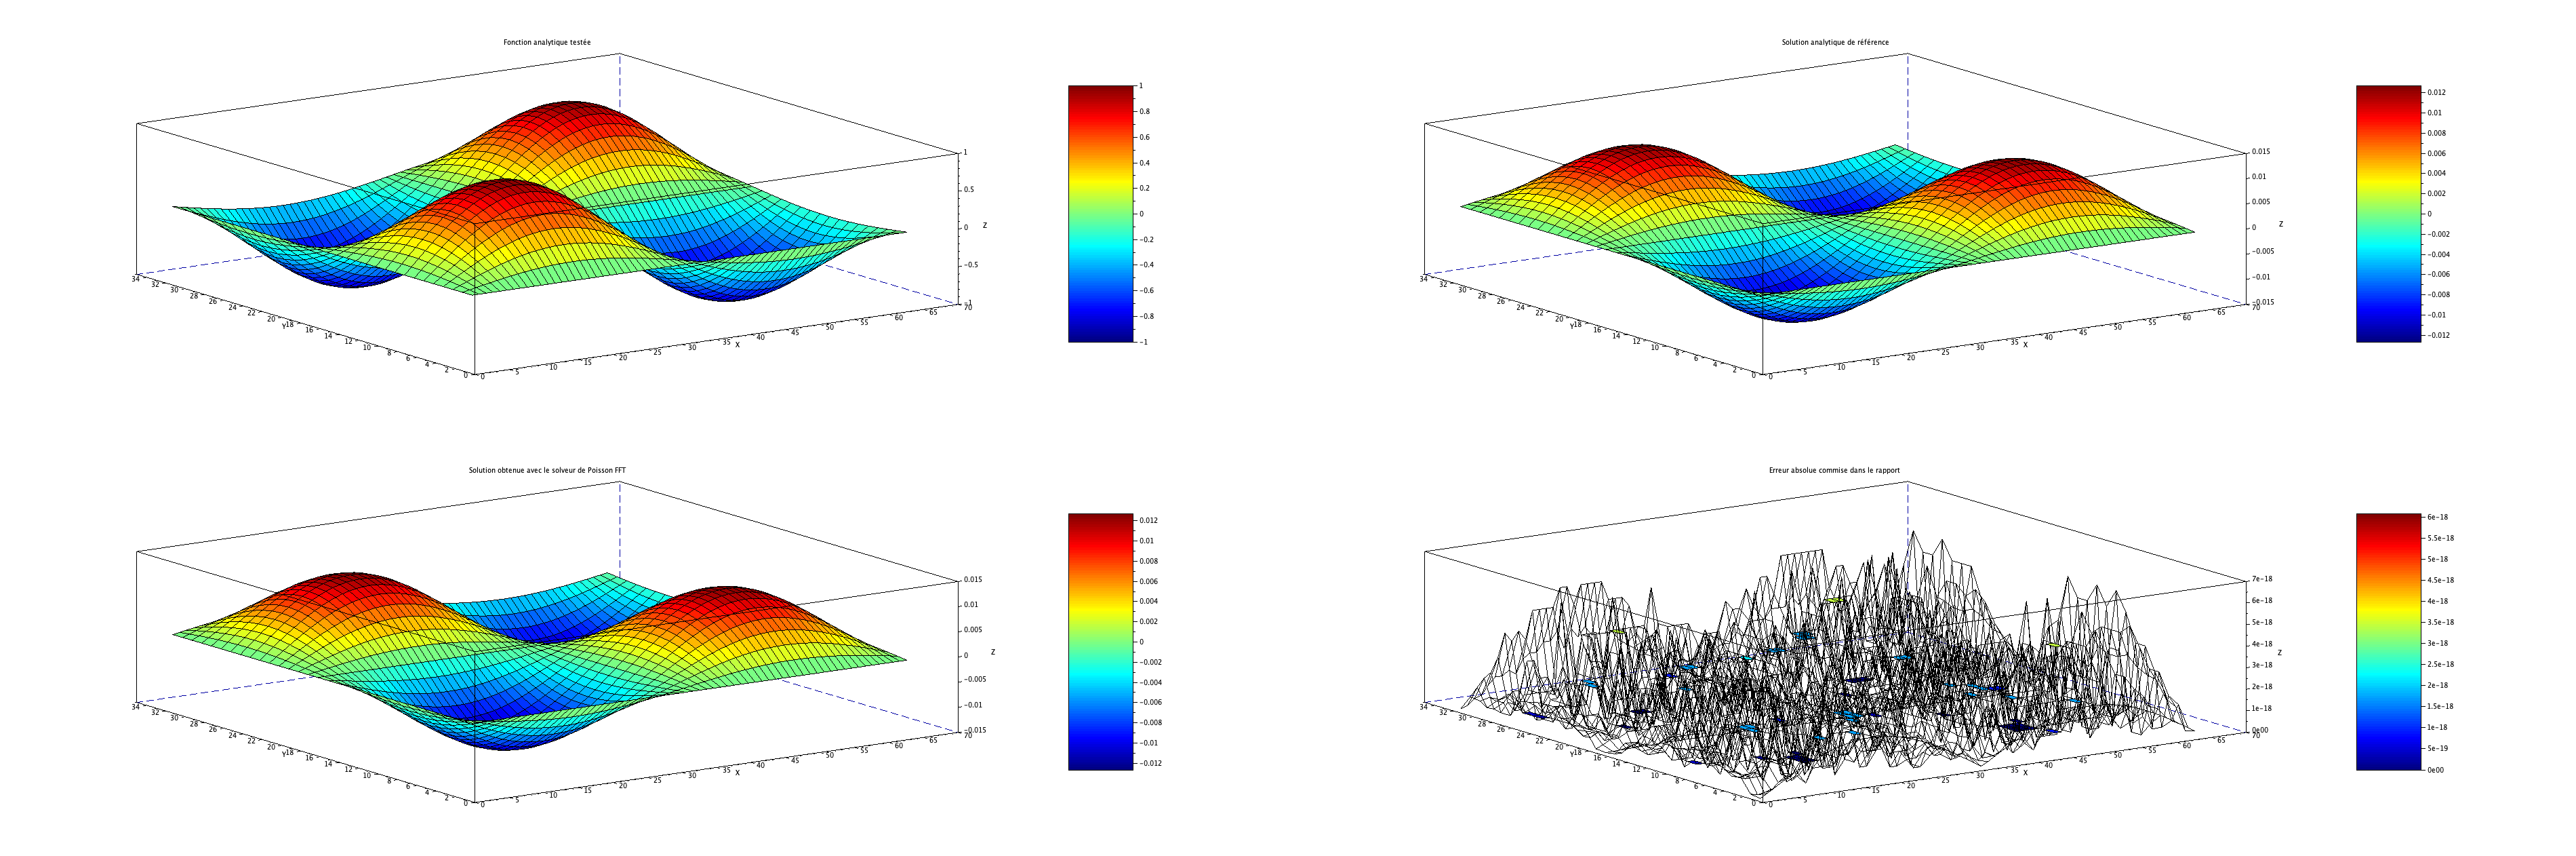
\includegraphics[scale=0.2]{poisson_error.png}
\captionof{figure}{Résultat de la simulation.}
\label{fig1}
\end{center}
\vskip 0.5cm
\textbf{On constate pour la fonction analytique testée que la solution obtenue par le solveur du poisson-2d se concorde au graphe de la solution analytique de référence. A ce stade, on serait de conclure que le solveur est correct, néanmoins, pour conforter cette idée, il faut voir l'erreur absolue entre les deux.}
\vskip 1cm
\begin{center}
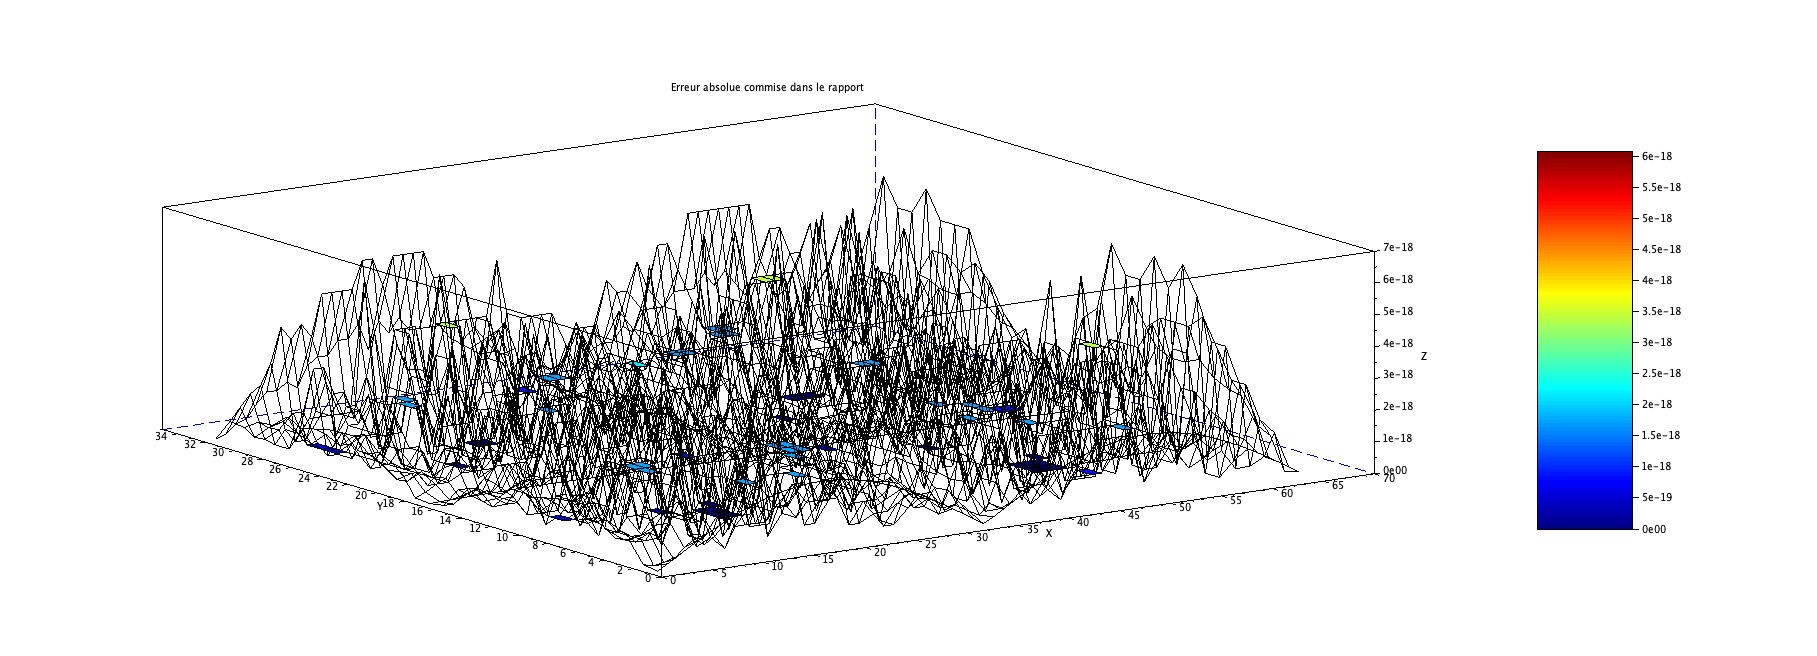
\includegraphics[scale=0.2]{error.png}
\captionof{figure}{Zoom sur l'erreur}
\label{fig1}
\end{center}
\textbf{L'erreur absolue ne dépasse pas  7e-18, qui est une valeur trop petite. On peut alors conclure que le solveur poisson-2d donne des résultats corrects et vraisemblables.}
\end{question}
\vskip 0.5
\begin{question}
Le résultat de la simulation est le suivant:
\begin{center}
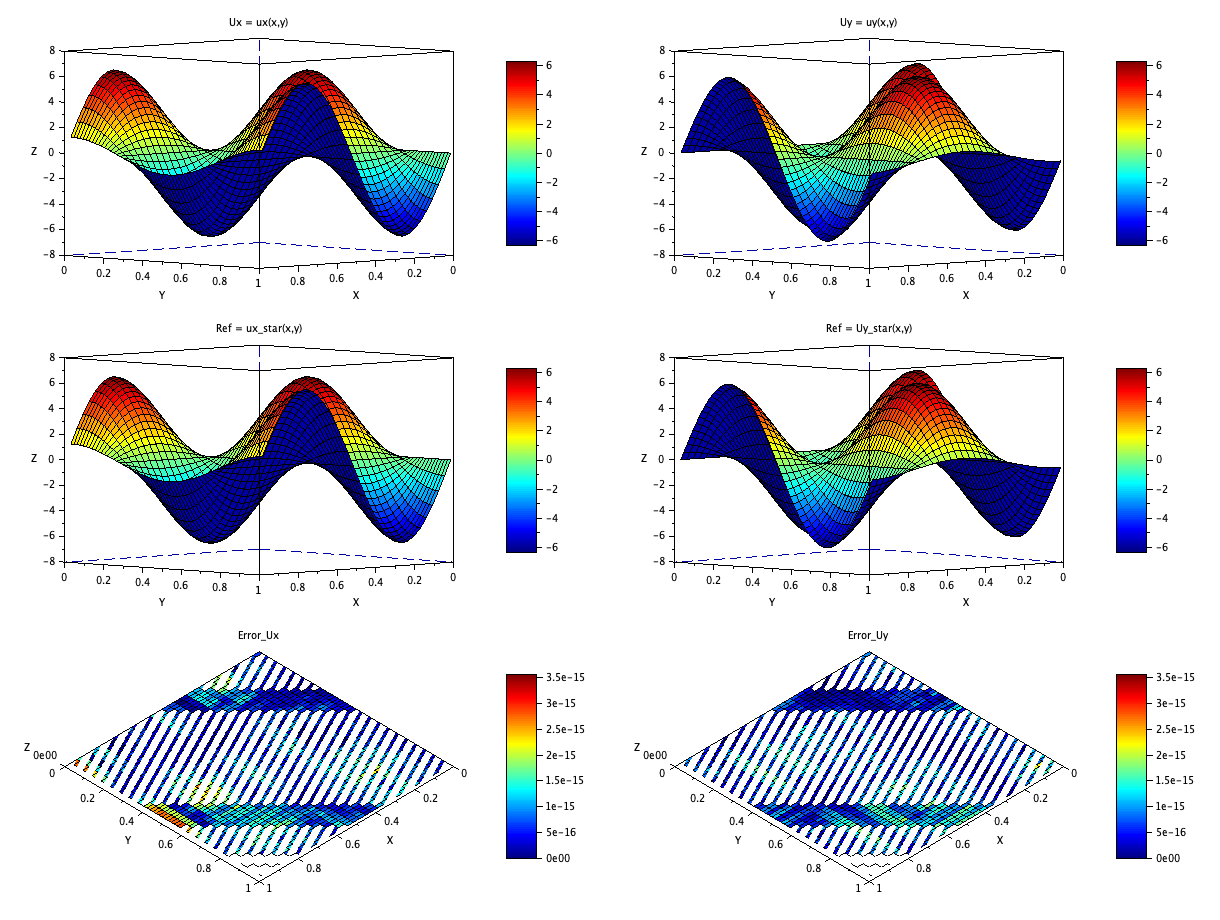
\includegraphics[scale=0.35]{poisson_error_curl.png}
\captionof{figure}{Résultat de la simulation.}
\label{fig1}
\end{center}
\vskip 0.5cm
\textbf{La solution de la simulation du solveur poisson-curl-2d s'apparente aux graphes des références.Voyons alors l'erreur absolue pour conclure sur l'efficacité de ce dernier.}
\vskip 1cm
\begin{center}
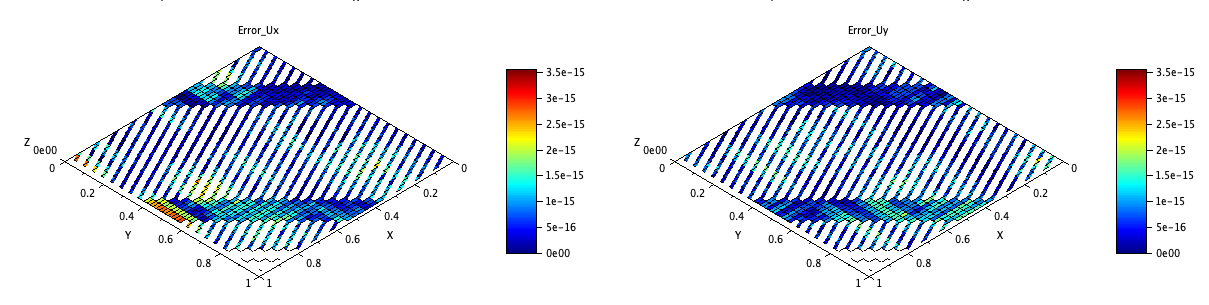
\includegraphics[scale=0.35]{erreurs_curl.png}
\captionof{figure}{Zoom sur les erreurs de Ux et Uy}
\label{fig1}
\end{center}
\vskip 0.5cm
\textbf{L'erreur pour Ux et Uy ne dépasse pas 4e-15, mais reste plus grande que celle de la question d'avant, ce qui est normal vu que ce solveur a plus d'opérations à  processer (une dérivation de plus) et en résulte du coup une baisse de la précision. Mais l'erreur obtenue reste suffisament petite pour conclure que le solveur donne des résultats logiques et vraisemblables.}
\vskip 1cm
\end{question}
\vskip 1cm
\section{ Simulation numérique}
\begin{question}
on calcule le champs de vorticité initial  $ \omega^{0}(x,y) = \frac{\partial u_y^0}{\partial x} - \frac{\partial u_x^0}{\partial y}$


on a

$$ \frac{\partial u_y^0}{\partial x} =
\begin{cases}
\rho (1 - \tanh^2(\rho [y - 0.25])) &\text{ si }y\leq  0.5  \\
 - \rho (1 - \tanh^2(\rho [0.75 - y ])) &\text{ si }y > 0.5
\end{cases}
$$

alors:
$$ \omega^{0}(x,y) =
\begin{cases}
2\pi \delta \sin(2 \pi x) - \rho (1 - \tanh^2(\rho [y - 0.25]))  &\text{ si }y\leq  0.5  \\
2\pi \delta \sin(2 \pi x) + \rho (1 - \tanh^2(\rho [0.75 - y ])) &\text{ si }y > 0.5
\end{cases}
$$
\end{question}
\vskip 8cm
\begin{question}
Les résultats de la simulation à t=0.80 et t=1.20
sont les suivants
\begin{center}
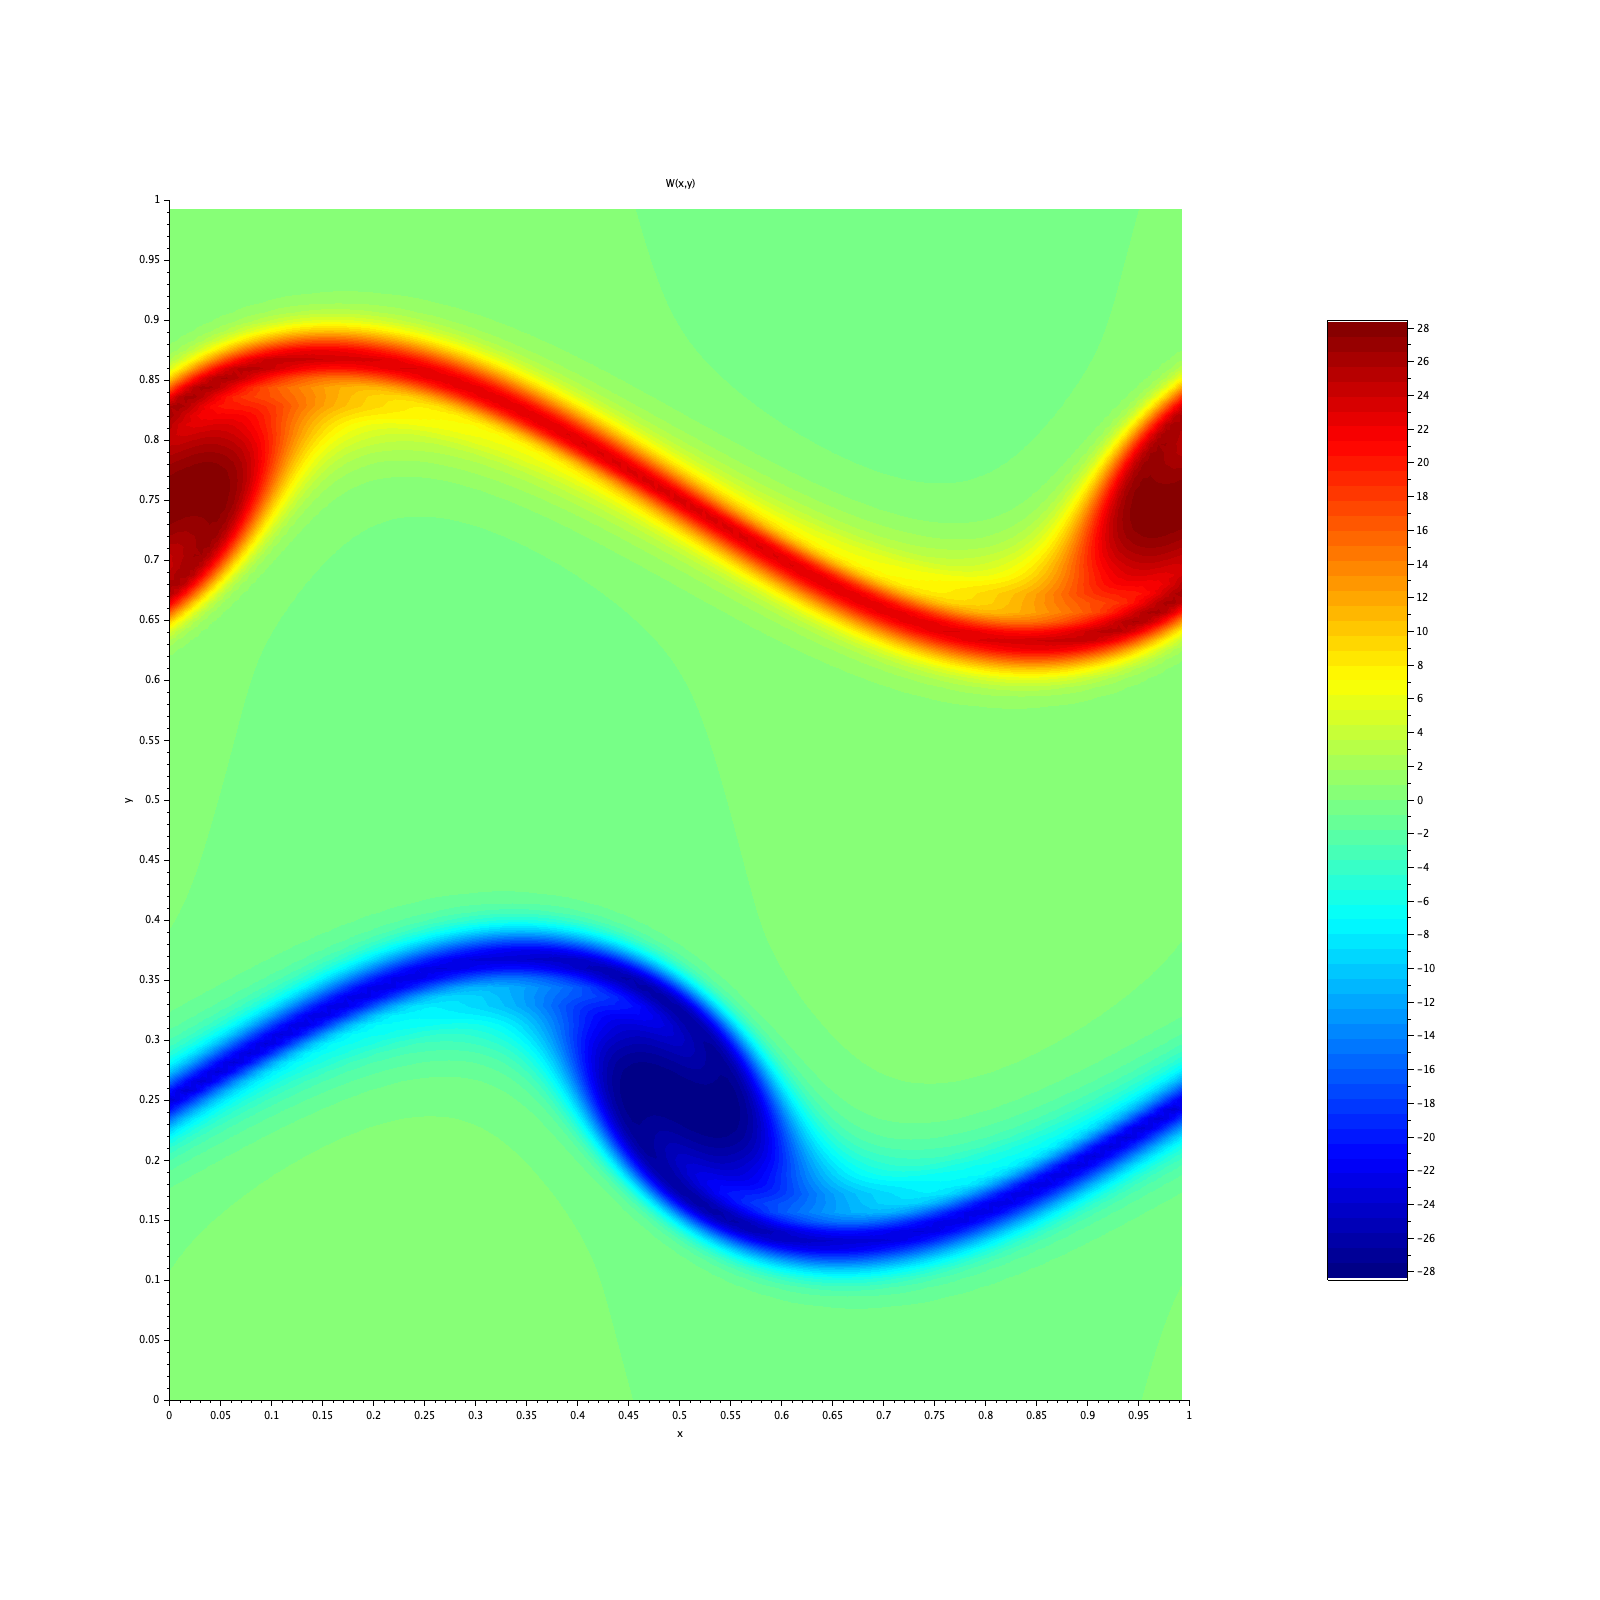
\includegraphics[scale=0.15]{isocontours_0,800000.png}
\captionof{figure}{Isocontours à t=0.80}
\label{fig1}
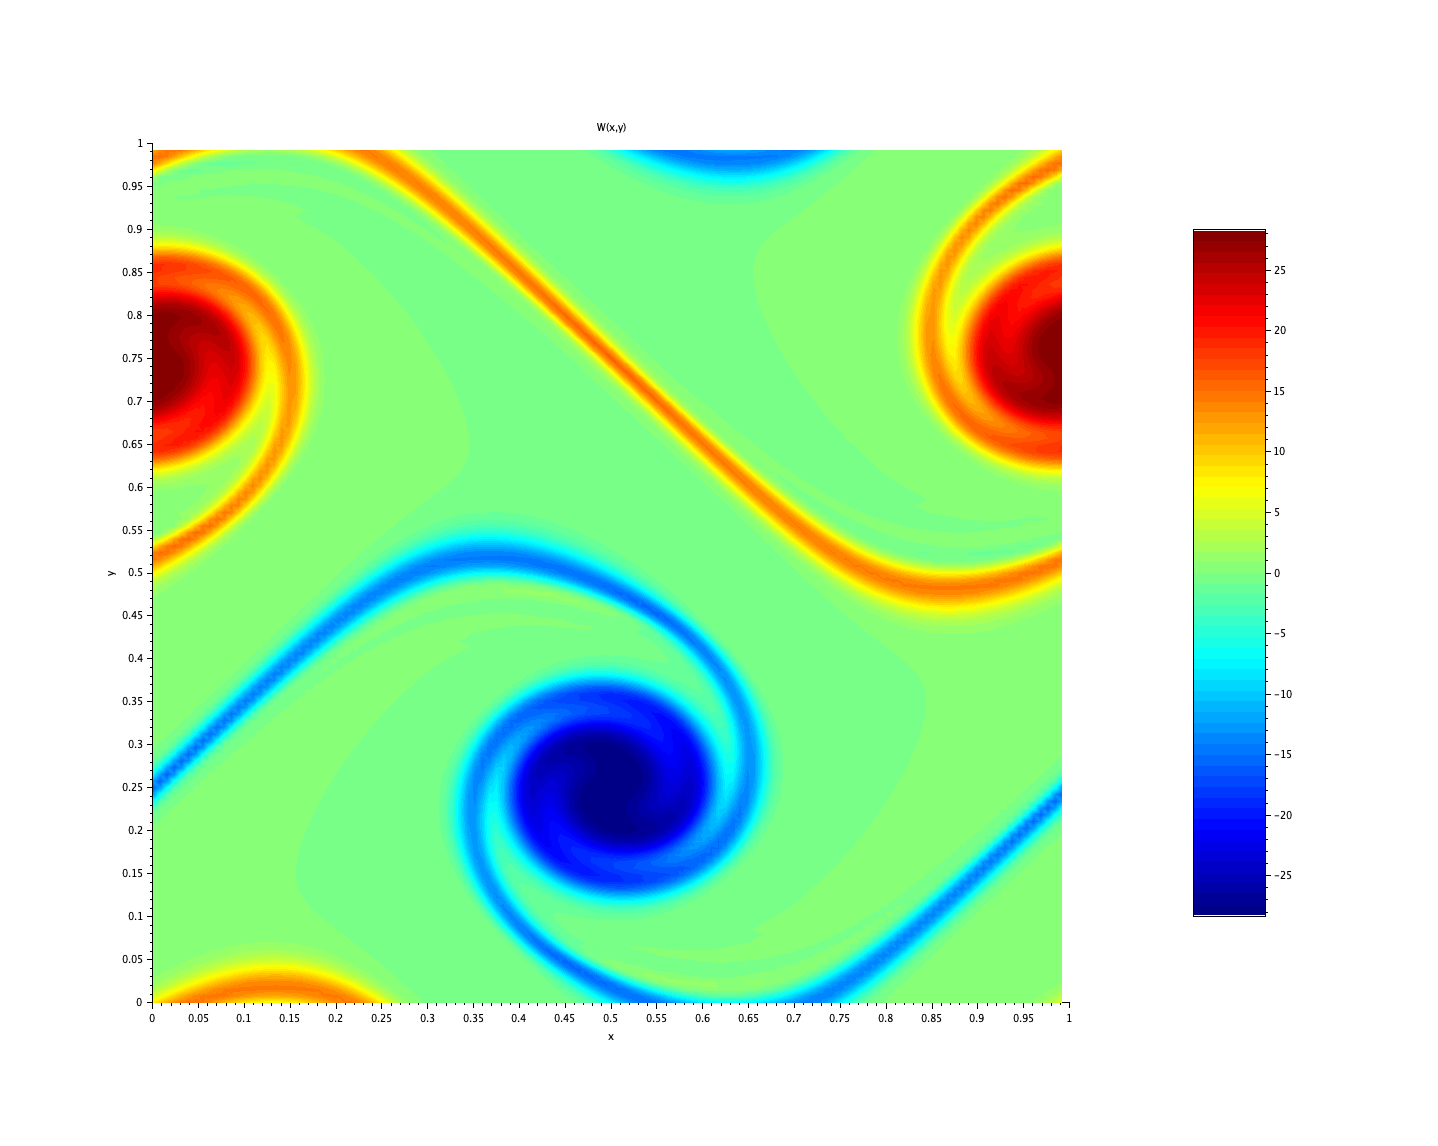
\includegraphics[scale=0.2]{isocontours_1,200000.png}
\captionof{figure}{Isocontours à t=1.20}
\label{fig1}
\end{center}
\textbf{On remarque dans la video (voir dossier teide) que plus on avance de le temps, plus la figure de W se distord pour créer une sorte de vortex qui rotate autour du point d'abscisse 0.5 et d'ordonnée 0.75.}
\vskip 1cm
Intéressons nous désormais aux isocontours:
\begin{center}
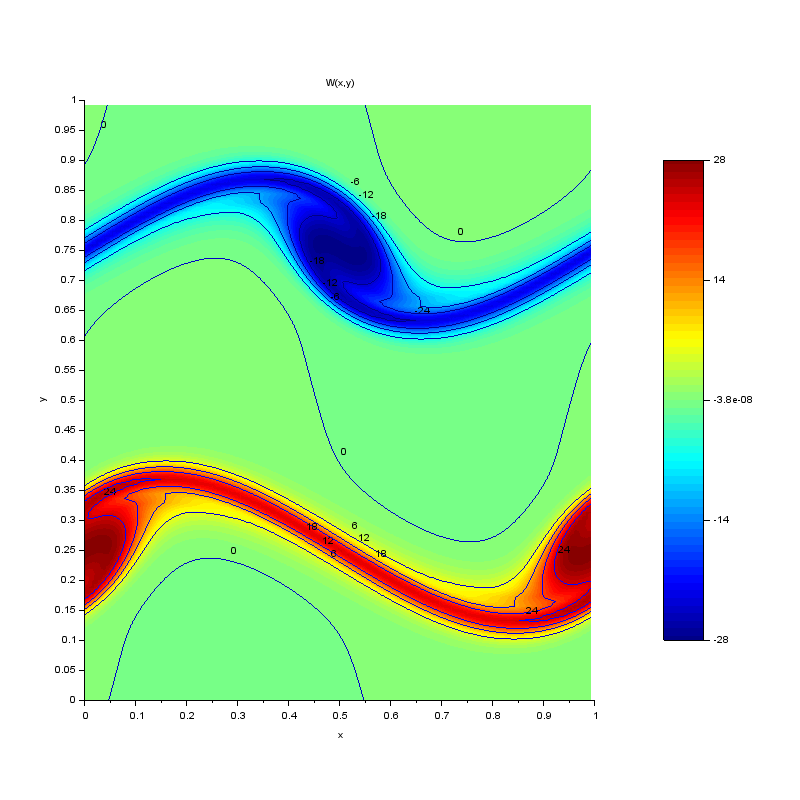
\includegraphics[scale=0.31]{iso80.png}
\captionof{figure}{Isocontours à t=0.80}
\label{fig1}
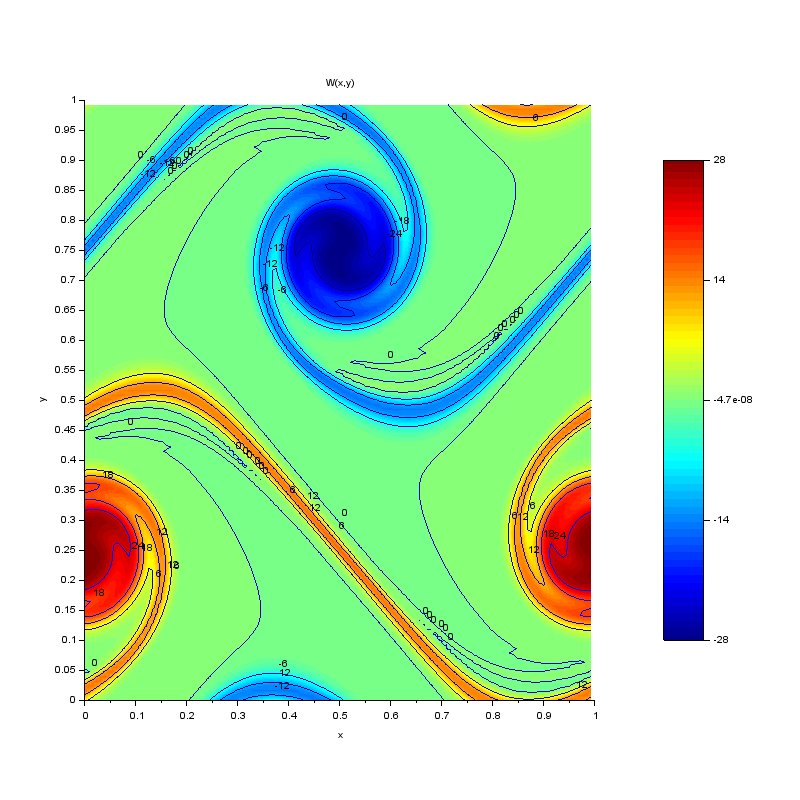
\includegraphics[scale=0.31]{iso120.png}
\captionof{figure}{Isocontours à t=1.20}
\label{fig1}
\end{center}
\vskip 0.5cm
\textbf{Quand on étudie les isocontours ci dessus, on trouve que les résultats concordent avec ce qui a été trouvé précedemment.}
\end{question}
\vskip 1cm
\begin{question}
On réitére la même simulation avec des paramètres différents.
\vskip 0.2cm
On trouve les résultats suivants:
\begin{center}
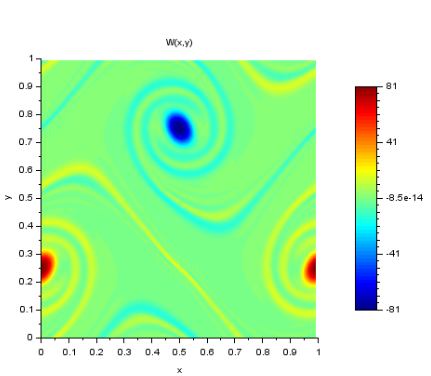
\includegraphics[scale=0.5]{isocontour_0,80.png}}
\captionof{figure}{Isocontours à t=0.80}
\label{fig1}
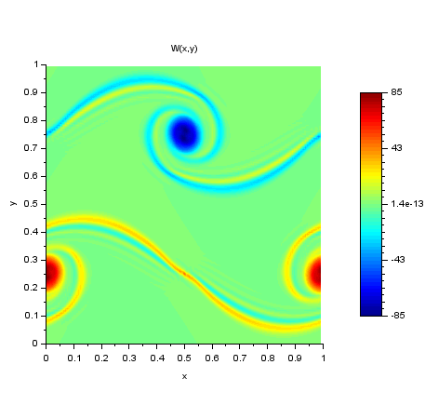
\includegraphics[scale=0.5]{isocontour_1,20.png}}
\captionof{figure}{Isocontours à t=1.20}
\label{fig1}
\end{center}
\vskip 1cm
\textbf{On remarque que avec ces paramètres le vortex se crée plus rapidement
mais conserve le même point central de rotation.
On en déuit donc que ce point central dépend des conditions initiales.Aussi, on observe une certaine périodicité spatiale qui concorde bien avec notre modèle.
Ce paramétrage prend beaucoup plus de temps car son nombre d'itérations est bien supérieur à celui du précédent.
\vskip 0.4cm
Le résultat est donc satisfaisant.}
\vskip 7cm
Quand aux isocontours cette fois on trouve:
\begin{center}
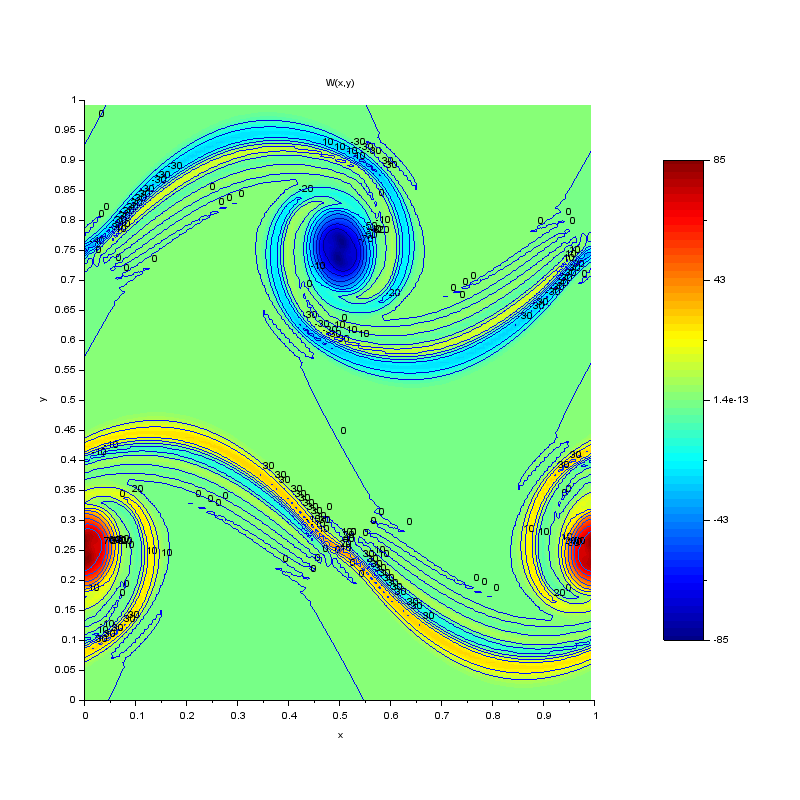
\includegraphics[scale=0.29]{iso802.png}}
\captionof{figure}{Isocontours à t=0.80}
\label{fig1}
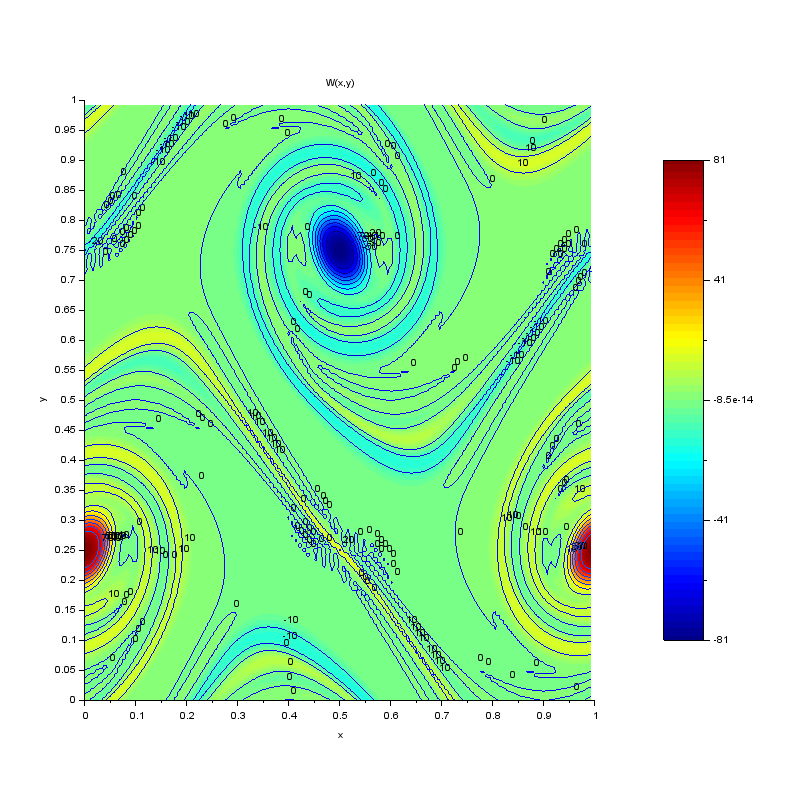
\includegraphics[scale=0.29]{iso122.png}}
\captionof{figure}{Isocontours à t=1.20}
\label{fig1}
\end{center}
\vskip 0.4cm
\textbf{N.-B: Vu que cette simulation prend beaucoup plus de temps que la précédente, ses résultats ont été supprimés pour ne pas alourdir le dossier à rendre. Ainsi, le script simu est paramétré selon la question 13.}
\end{question}
\vskip 2cm
\begin{question}
\end{question}

\end{document}
